\documentclass[presentation]{subfiles}

\onlyinsubfile{
}
\begin{document}

\subfile{threads}
% \againframe<2>{threads}

\begin{frame}{Complexity}
  \begin{columns}
    \begin{column}{.6\textwidth}
      \visible<-4>{What do we mean when we say \alert{complexity}?}
    \end{column}
    \begin{column}{.4\textwidth}
      \only<5->{\hfill \dots~In some cases. Sometimes.}
    \end{column}
  \end{columns}
  \begin{columns}
  \begin{column}{.55\textwidth}
  \begin{itemize}
    \item<2-> Can crowds help you \alert{revise} work?\par
    \scriptsize{\textcite{bernsteinSoylent,Kim:2014:CSI:2556288.2556986,Nebeling:2016:WCW:2858036.2858169}\par}\normalsize{}
    \item<3-> Can crowds \alert{critique} designs?\par
    \scriptsize{\textcite{yuanAlmost,fuge2014analysis}\par}\normalsize{}
    \item<4-> Can crowds create artifacts \alert{de novo}?\par
    \scriptsize{\textcite{KimStoria,Kim2017,Hahn:2016:KAB:2858036.2858364,Lasecki:2014:LSR:2661334.2661352}\par}\normalsize{}
  \end{itemize}
  \end{column}
  \begin{column}{.45\textwidth}
      \begin{itemize}
        \item[$\Rightarrow$]<6-> \hfill With variable success\par
        \visible<0>{\scriptsize{\textcite{bernsteinSoylent,Nebeling:2016:WCW:2858036.2858169}\par}\normalsize{}}
        \item[$\Rightarrow$]<7-> \hfill With careful guidance\par
        \visible<0>{\scriptsize{\textcite{yuanAlmost,fuge2014analysis}\par}\normalsize{}}
        \item[$\Rightarrow$]<8-> \hfill Within narrow specifications\par
        \visible<0>{\scriptsize{\textcite{Hahn:2016:KAB:2858036.2858364,Lasecki:2014:LSR:2661334.2661352}\par}\normalsize{}}
      \end{itemize}
  \end{column}
  \end{columns}
\end{frame}


\begin{frame}{What Does On--Demand Work Say?}
  \begin{columns}
    \begin{column}{0.5\textwidth}
      Build complexity into the process
      \begin{itemize}
        \item<+-> Apply CS methods to people\par
                 \scriptsize{\textcite{crowdForgeKittur}\par}\normalsize{}
        \item<+-> Humans as computational units\par
                 \scriptsize{\textcite{Lasecki:2014:LSR:2661334.2661352}\par}\normalsize{}
        \item<+-> Crowdsourcing workflows as function state machines\par
                 \scriptsize{\textcite{latoza2014microtask}\par}\normalsize{}
      \end{itemize}
    \end{column}
    
    \begin{column}{0.5\textwidth}
      \only<1>{
      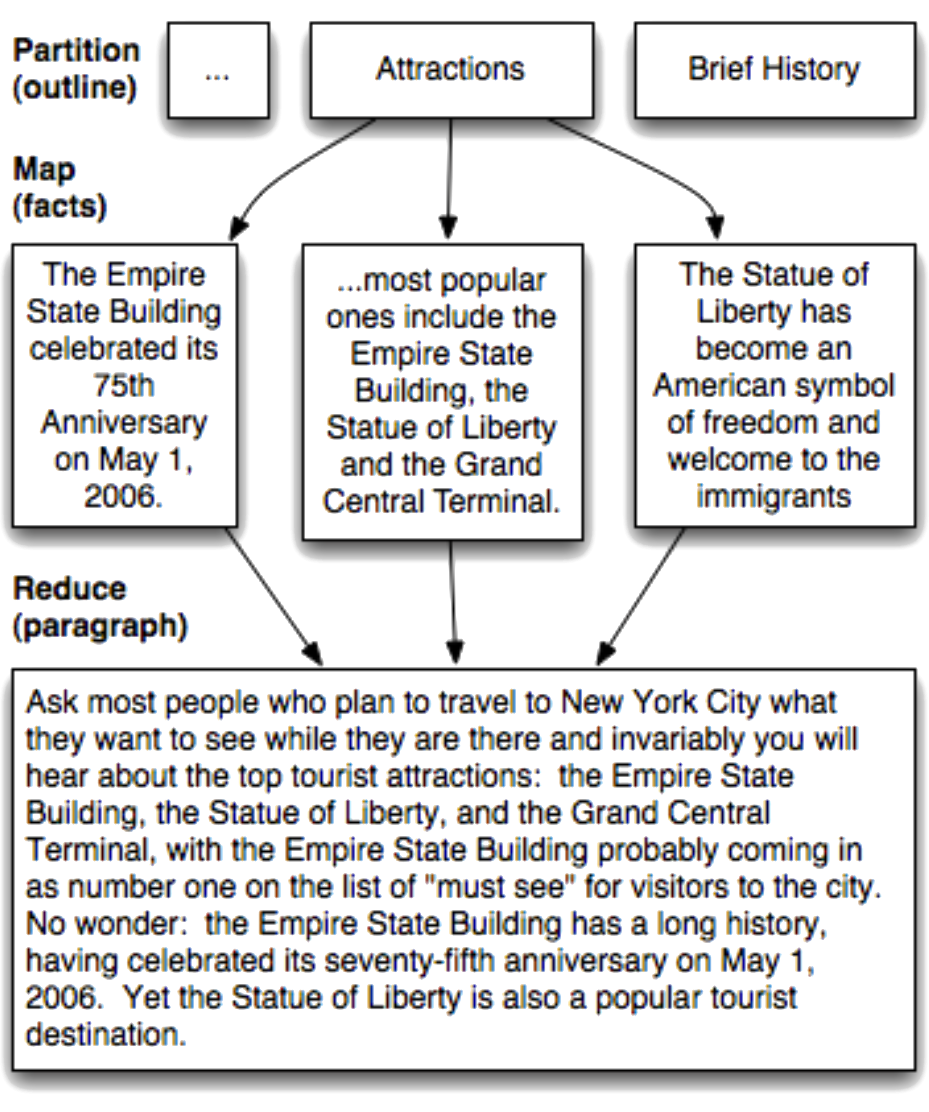
\includegraphics[max width=\textwidth,max height=.9\textheight]{figures/complexity/cw_literature/mapReduce.png}
      }
      
      \only<2>{
        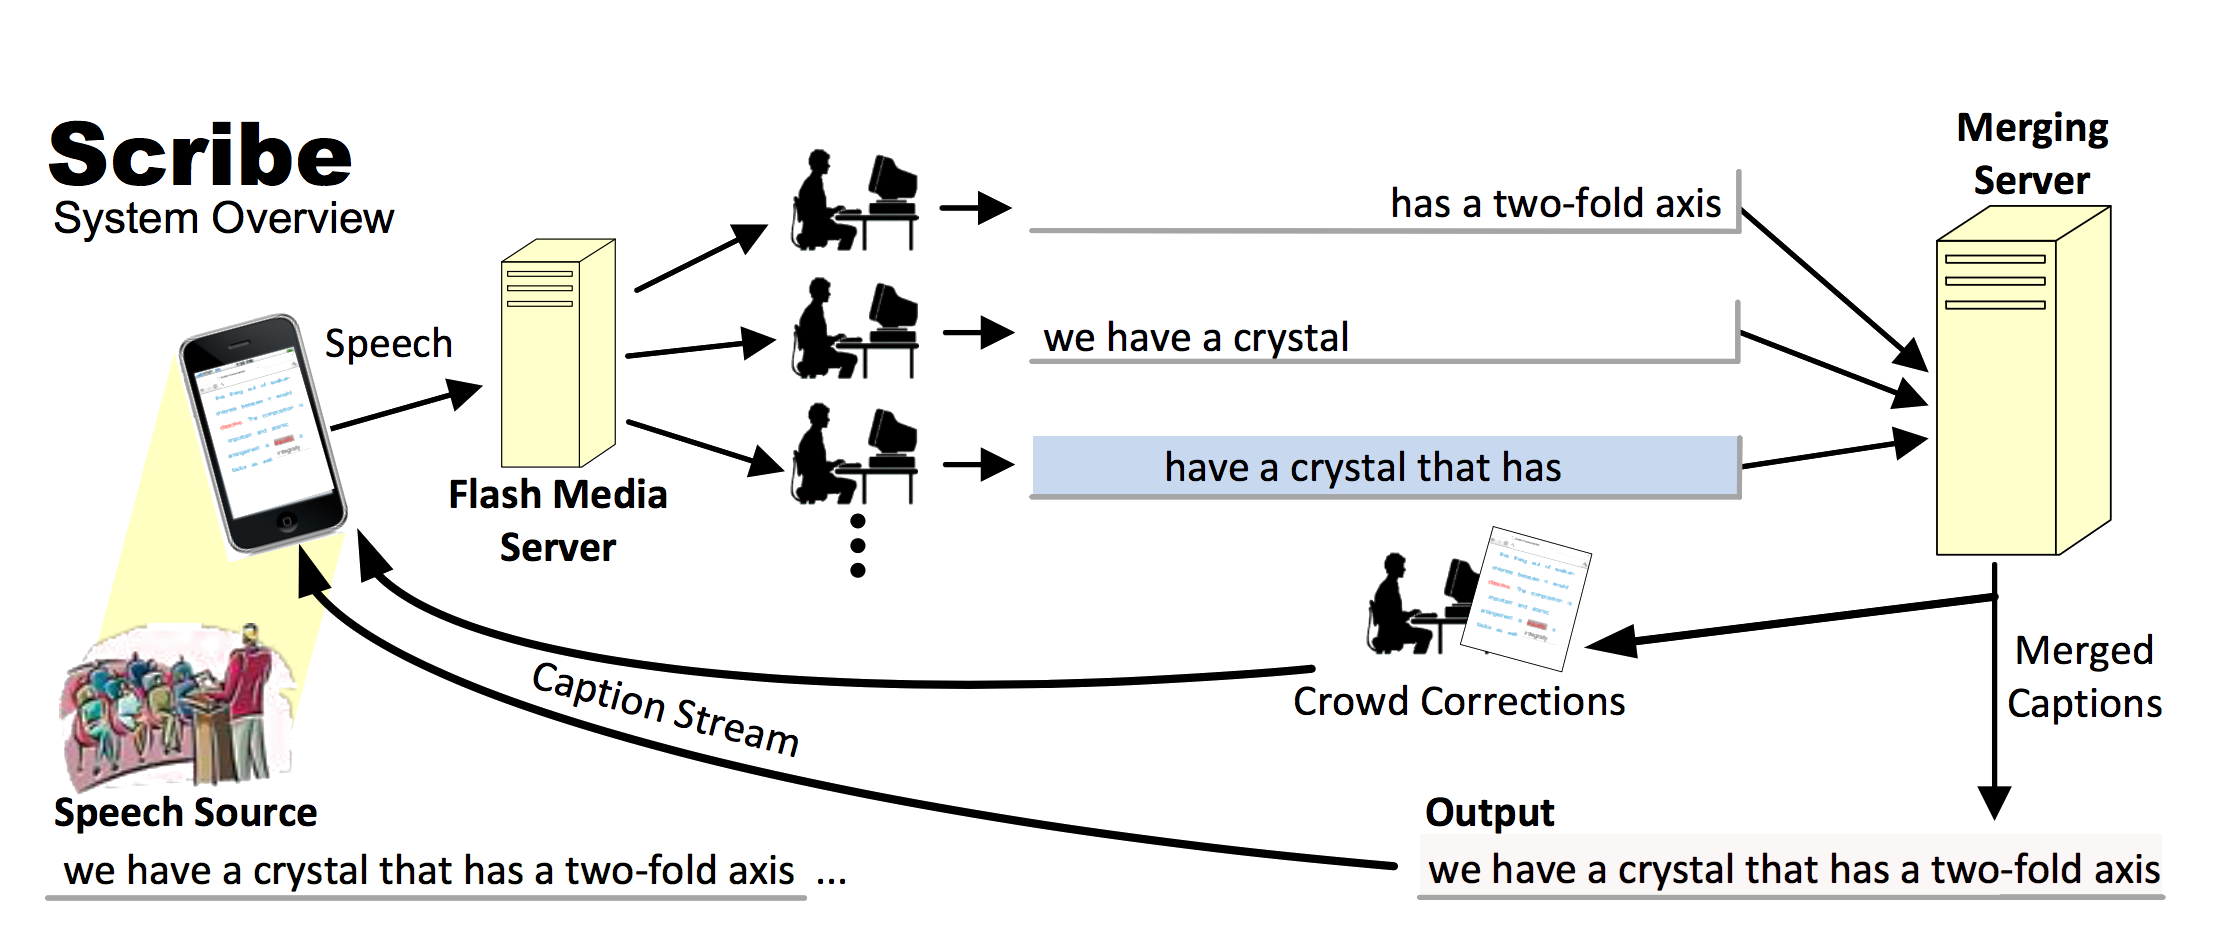
\includegraphics[max width=\textwidth,max height=.7\textheight]{figures/complexity/cw_literature/scribe.png}
      }
      \only<3>{
        \begin{adjustbox}{max totalsize={\textwidth}{.9\textheight},center}
        \begin{tikzpicture}[->,>=stealth',auto, node distance=4cm,
                            thick,transform shape]
          \node[state,label=above:{Described}]                       (A)                    {};
          \node[state,label=left:{Described written}]                (B) [below of=A]       {};
          \node[state,label=left:{Run Tests}]                        (D) [below of=B]       {};
          \node[state,label=below:{Described written buggy}]         (C) [below right of=D] {};
          \node[state,label=below:{Described written buggy}]         (E) [below left of=D]  {};

          \path[every node/.style={sloped,anchor=south}]
                (A) edge              node {Write description} (B)
                (B) edge [loop right] node {Edit code} (B)
                    edge              node {Edit code} (D)
                (D) edge              node {} (C)
                    edge              node {} (E)
                (C) edge [bend right] node {Debug} (B)
                    edge [bend right] node {Debug} (D)
                (E) edge [bend right] node {Edit Code} (D)
                    edge [bend left]  node {Edit Code} (B);
          \end{tikzpicture}
          \end{adjustbox}
      }
    \end{column}
  \end{columns}
\end{frame}

\begin{frame}{What Does Piecework Say?}
  What we'll find
  \begin{itemize}
    \item<+-> Building complexity into the processes
    \item<+-> Incremental advances until managers \emph{tracked} and \emph{standardized} workers and work
    \item<+-> Insights into task specialization
  \end{itemize}
\end{frame}

\begin{frame}[t]{What Does Piecework Say?}
      George Airy (astronomer) used a very similar approach\par
      \scriptsize{\textcite{grier2013computers}\par}\normalsize{}
    \begin{columns}
    \begin{column}{0.6\textwidth}
      \begin{figure}
        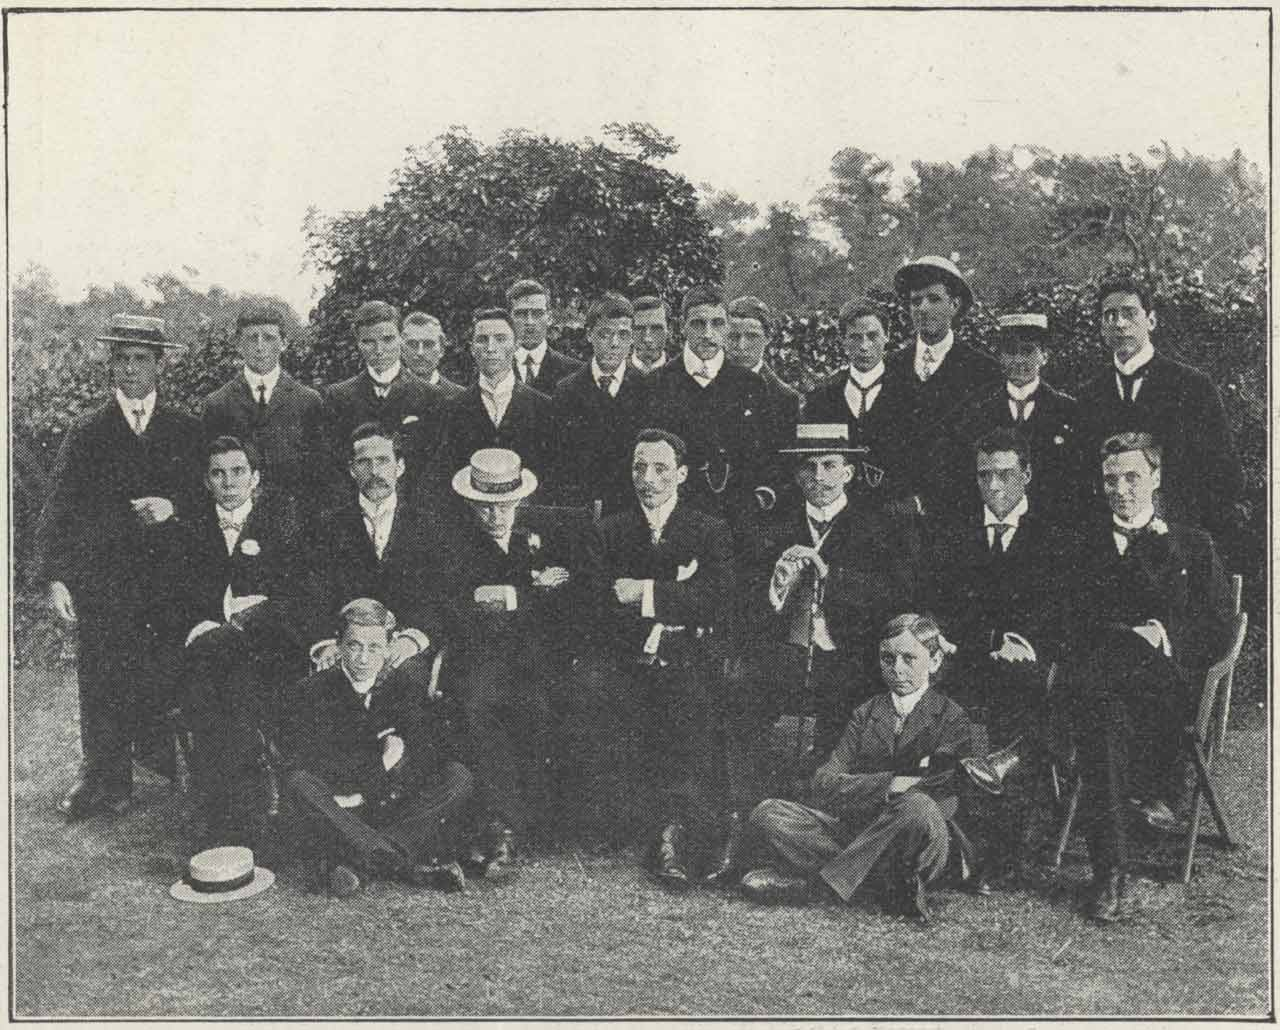
\includegraphics[max width=\textwidth, max height=.7\textheight,keepaspectratio]{figures/photo/Greenwich-Observatory-computing-staff-1902.jpg}
      \end{figure}
    \end{column}
    
    \begin{column}{0.4\textwidth}
      \begin{itemize}
        \item Employed computers
        \item 13--20 years old
        \item no particularly strong background in mathematics
        \item A basic understanding of logarithms, algebra, etc\dots
      \end{itemize}
    \end{column}
    \end{columns}

\end{frame}


\begin{frame}{George Airy}
    Airy built complexity into the process, assigning \emph{human computers} 
    to calculate \& verify the \emph{right ascension} and \emph{declination} of stars.

    \begin{figure}
    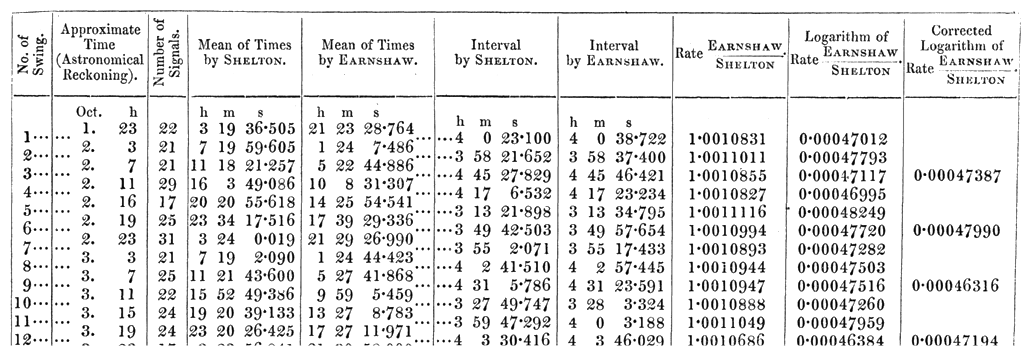
\includegraphics[width=\textwidth]{figures/complexity/pw_literature/airy.png}
    \end{figure}
\end{frame}


\subfile{piecework-simple}
\subfile{piecework-complex}


\begin{frame}{Comparisons}

\begin{itemize}
    \item<+-> Building complexity into the processes
    % \item<+-> Incremental advances until managers \emph{tracked} and \emph{standardized} workers and work
    % \item<+-> Insights into task specialization
  % \end{itemize}
% \begin{itemize}
  \item Challenges dealing with flexibility
  \begin{itemize}
    \item \emph{Building} planes versus \emph{fixing} trains
  \end{itemize}
\end{itemize}
\end{frame}

\begin{frame}{Implications for On--Demand Work}
  Has technology shifted on--demand work?
    \begin{itemize}
      \item Technology makes \emph{some} complex tasks relatively trivial
      \item Measuring workers is easier than ever
    \end{itemize}
\end{frame}


\begin{frame}{Enhanced Cognition} % {Cab Drivers}
  \begin{figure}
  \includegraphics<1>[width=\textwidth]{figures/photo/knowledge-student.jpg}
  \only<2>{
  % \begin{columns}
  % \begin{column}{0.2\textwidth}
  % 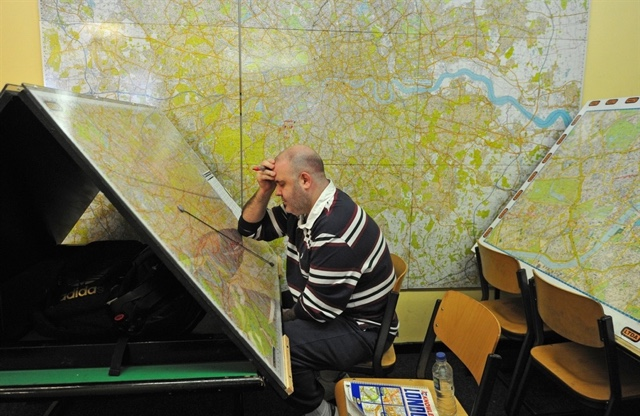
\includegraphics[width=\textwidth]{figures/photo/knowledge-student.jpg}
  % \end{column}
  % \begin{column}{0.8\textwidth}
  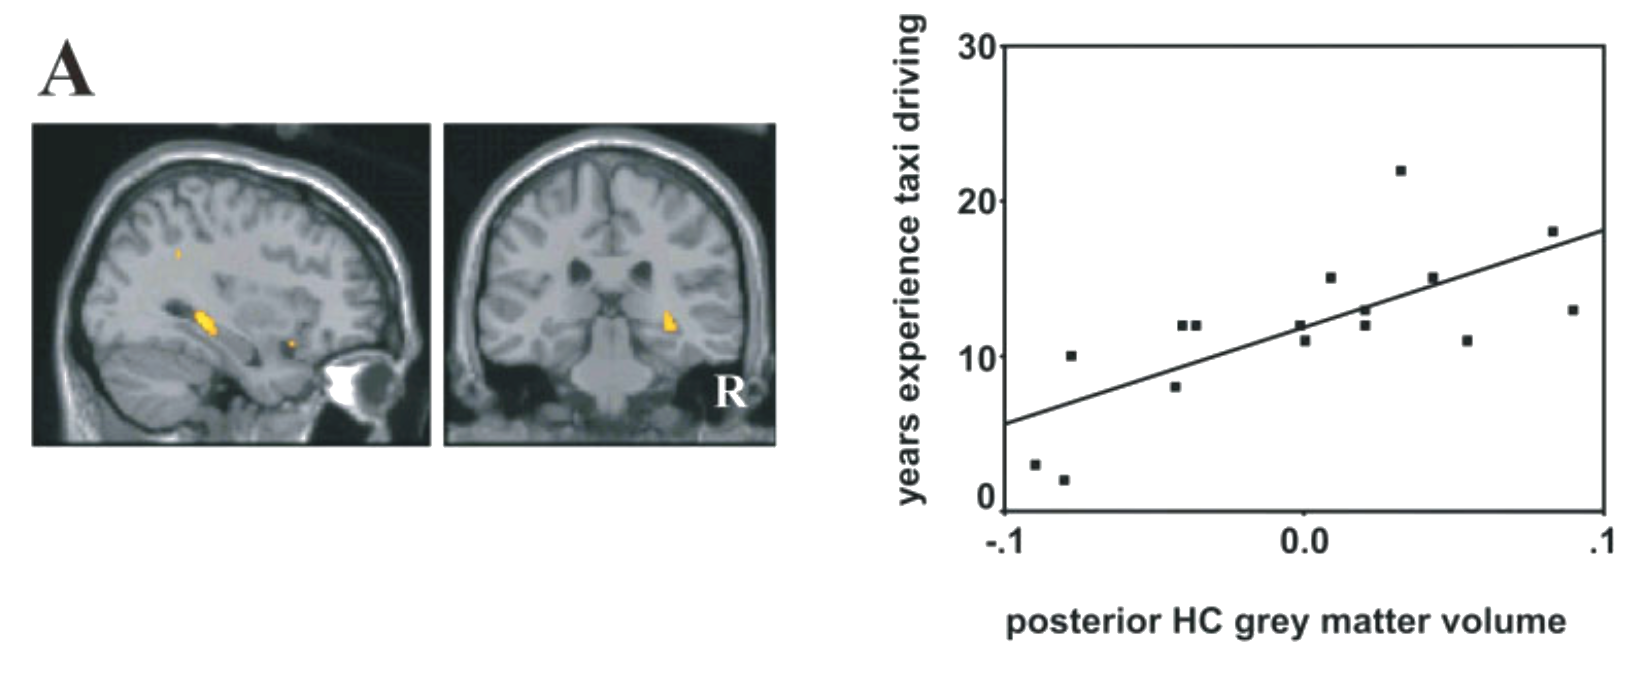
\includegraphics[width=\textwidth]{figures/complexity/brain_scansA.png}
  % \end{column}
  % \end{columns}
  }
  \includegraphics<3>[width=\textwidth]{figures/photo/gps-map.jpg}
  \end{figure}
\end{frame}

\begin{frame}{Tracking Work and Workers} % {Algorithmic Measurement}
\begin{columns}
\begin{column}{.5\textwidth}
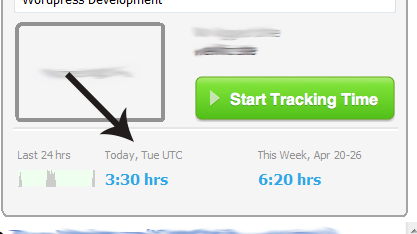
\includegraphics[max width=\textwidth,max height=.8\textheight,keepaspectratio]{figures/screenshot_odeskteamapp.jpg}
\end{column}
\begin{column}{.5\textwidth}
% \begin{itemize}
  Upwork has turned to logging workers' keystrokes and taking screenshots automatically every 10 minutes
% \end{itemize}
% 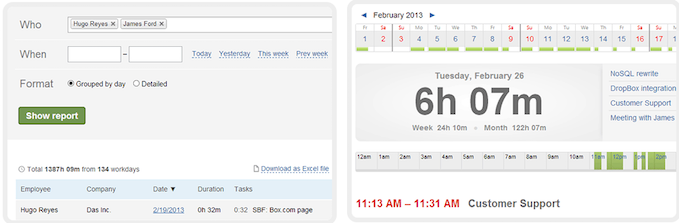
\includegraphics[max width=\textwidth,max height=.8\textheight,keepaspectratio]{figures/time-tracking-like-odesk-screenshot-monitor1.png}
\end{column}
\end{columns}

    % notes
    % \begin{itemize}
      % \ali{Upwork's screen recording tool as a way to measure workers}
      % \item also maybe google analytics and other ways of tracking web--based workers
    % \end{itemize}
\end{frame}

\begin{frame}{Takeaways}
  \begin{itemize}
    \item We make stronger assumptions about workers' abilities thanks to technology
    \item Evaluation remains difficult, but we're trying to find stopgap solutions through decomposition
    \item We're still not solving the problems of inherently subjectively judged work
  \end{itemize}
\end{frame}

% \onlyinsubfile{
%   \printbibliography{}
% }
\end{document}